

\chapter{Classes for images}


%---------------------------------------------
%---------------------------------------------
%---------------------------------------------

\section{Introduction}

Also \PPP is not specifically an image processing library, there are several parts where
image are used to extract information (for example target detection) or as data helpfull 
for other processing (for example tabulating function for fast access) and, 
at the end, image manipulation is a non neglectable part
of the code.
This chapter describe the general organization of image processing code.

By some historical language abuse we call \emph{image} what is now commonly called a tensor,
i.e. an array of $S_1 \times S_2 \times \dots S_d$ values , where $d$ is the dimension
of the image, $S_1$, $S_2$ \dots the sizes in each dimension.




%---------------------------------------------
%---------------------------------------------
%---------------------------------------------
\section{Files organization }

We begin by a description of files and folder related to images.

%----------------------------------------------------------------------------------------

\subsection{Connected files}

Note the following files that are not directly image files, but are strongly connected :

\begin{itemize}
	\item {\tt MMVII\_Ptxd.h} contain the definition of points, and consequently of pixels (point
		with integers coordinates),  contains the definition of boxes (and images inherit
		of boxes);

	\item {\tt MMVII\_Matrix.h} dense vector and dense matrix can be regarded as images ($1$ or $2$ dim), so in \PPP
		they are implemented as a shell arround  images of dimension $1$ or $2$
\end{itemize}


%----------------------------------------------------------------------------------------

\subsection{Header files}


The file containing classes for representing images are essentially :

\begin{itemize}
	\item {\tt MMVII\_Images.h} this file contain the classes for representing 
		generic images indepently of their dimension;
		it contains also the classes specific to images of dimension $1$ and $3$,
		which play a role less important then $2d$ images;

	\item {\tt MMVII\_Image2D.h} this file contain the classes specific to $2$-dimensionnal
              images which obviously are the more frequent and more devlopped.
\end{itemize}


The definition (ie the code) of image processing routines can be found in "cpp" files
(for "big" routines) or inlined in header files (for "small" routines).
The declaration of routines defined in cpp files are found in :

\begin{itemize}
	\item {\tt MMVII\_Linear2DFiltering.h} contain linear filters , they are essentially
		gaussian filters routines and class for gaussian pyramid (for sift-like multiscale);

	\item {\tt MMVII\_NonLinear2DFiltering.h} contains declaration of non linear filters (for
		now their implemantation will often use  V1);

	\item {\tt MMVII\_ImageInfoExtract.h} contains declaration of classes and routines
		for information extraction, for now contains fast extremum extraction,
		and routine for extracting connected component on black and white image

	\item {\tt MMVII\_ExtractLines.h} contains declaration of classes and routine for 
		line extraction (hough transform);
\end{itemize}


The following header files contains direcly the code of the function they implemant :

\begin{itemize}
	\item {\tt MMVII\_TplGradImFilter.h} contains code for gradient with optimization
		(by tabulation) for fast computation of polar decomposition 

        \item {\tt MMVII\_TplImage\_PtsFromValue.h} contain a very specific function for extracting
	      a point having a given value in an image (used for target "fine" detection);

      \item {\tt MMVII\_Tpl\_Images.h} containd codes for global basic operation on images not
	      related to spatial organization  (i.e operation that can be defined using just
		a vector of values); as they are not using spatial relation it contains also matrix
		operation; example  difference, sum, conversion , multiplication by constant,  reduction
		(sum of elements, bounds); 

	\item {\tt MMVII\_TplSimpleOperator.h} a tentative to implemant a library similar to V1 for genericity,
		but using templatization rather than virtualization; will see if it is devloped ...
	
	\item {\tt MMVII\_TplSymbImage.h} used when image are used in non linear optimization, see \ref{ImageOptDiff}

\end{itemize}

%----------------------------------------------------------------------------------------

\subsection{Cpp files}

The {\tt cpp} files can be found in the following folders :

\begin{itemize}
     \item {\tt ImagesBase/} contains the definition of image classe, it correspond to 
	     essentially to declaration of {\tt MMVII\_Images.h} and {\tt MMVII\_Image2D.h} 

     \item {\tt ImagesFiltrLinear/} contains linear filtering definition , correpond to declaration of
	     {\tt MMVII\_Linear2DFiltering.h}, and also some final command (to move ?);

     \item {\tt ImagesInfoExtract/}  contains the code definition for \emph{low level} "object" extraction
\end{itemize}

%---------------------------------------------
%---------------------------------------------
%---------------------------------------------

\section{Numerical types}

\label{NumericalType}

In {\tt MMVII} the following numerical types are defined in  {\tt MMVII\_AllClassDeclare.h}


\begin{itemize}
    \item {\tt tREAL4}, {\tt tREAL8} , {\tt tREAL16} for floatting point values on
	    $4,8$ and $16$ bytes;

    \item {\tt tINT1}, {\tt tINT2} , {\tt  tINT4}, {\tt  tINT8} for signed integer types
	    on $1,2,4$ and $8$ bytes;

    \item {\tt tU\_INT1}, {\tt tU\_INT2} , {\tt  tU\_INT4}, {\tt  tU\_INT8} for signed integer types
            on $1,2,4$ and $8$ bytes;
\end{itemize}



%---------------------------------------------
%---------------------------------------------
%---------------------------------------------

\section{General image organization}

%----------------------------------------------------------------------------------------

\subsection{Parameter of image classes}

A class of image is parametrized by $2$ elements :

\begin{itemize}
   \item the type on which is coded each elements , it must be one of the numerical types
	   defined in \label{NumericalType};

   \item the dimension of the image,  the value can be $1$, $2$ or $3$ for now (there exist
	   also  unlimited dimension image, see ~\ref{UlimDimIm}  , but less efficient);
\end{itemize}


For maximal efficiency manipulation, the code must "know" the type and the dimension
of the image.  For example if we manipulate $2d$ images with integer element 
include in $[0,255]$:  we will use images of type {\tt cDataIm2D<tU\_INT1>},
and this class will contain a field {\tt mRawData2D} of type {\tt tU\_INT1 **}
such that the reference to the value of $1$ pixel can be extracted by   {\tt mRawData[y][x]}.
There exist aslo class {\tt cDataIm3D<Type>} containing a field {\tt mRawData3D} of type {\tt Type ***},
 and {\tt cDataIm1D} containing a field {\tt mRawData1D} of type {\tt Type *}.

Also some time it is interesting for limitating the size of code to maninuplate  images
independantly of their dimension or type. Sometime because this can be done as efficiently
as when we now the type and dimension, or sometime because effficiency is just not our priority. In
both case we avoid code duplication. This is the role of classes {\tt cDataTypedIm} and {\tt cDataGenUnTypedIm}.


The class {\tt cDataTypedIm<Type,Dim>} implement the code that can be written generically without using
the value of {\tt mRawData1D, mRawData2D, mRawData3D}.  Then {\tt cDataIm1D} inherits of {\tt cDataTypedIm<Type,1>},
{\tt cDataIm2D} inherits of {\tt cDataTypedIm<Type,2>} an {\tt cDataIm3D<Type>} inherits of class {\tt cDataTypedIm<Type,3>}.


The class  {\tt cDataGenUnTypedIm<Dim>} implement de  functionnality of images that can be written
independantly of the type of element used to store numerical values. The class {\tt cDataTypedIm<Type,Dim>}
inherits from {\tt cDataGenUnTypedIm<Dim>}.


%----------------------------------------------------------------------------------------

\subsection{Classes {\tt cDataGenUnTypedIm<Dim>}}


      %  -  -  -  -  -  -  -  -  - - - -  -  -  -  -  -  -  -  - -  -  -  -  -  -  -  -  -  - - - -  -  -  -  -  -  -  -  - -- 

\subsubsection{{\tt cDataGenUnTypedIm<Dim>} as rectangular objects }

The class {\tt cDataGenUnTypedIm<Dim>} is at the highest level in image  inheritance
hierachy.  Each {\tt cDataGenUnTypedIm<Dim>} is defined on a "rectangular" footprint
and consequently they inherit from class {\tt cPixBox<Dim>}. 

As a  {\tt cPixBox<Dim>}, all the pixels of a {\tt cDataGenUnTypedIm} can be parsed
using iterators, and code likes this one are current in {\tt MMVII} library :

\lstset {language=C++}
\begin{lstlisting}
   //  iterate all the pixel
   for (const auto & aP : aIm)
   {
        // do something with all pixel of image
   }

   // iterate all the pixel execpt bordder 3
   for (const auto & aPix : cRect2(mDIm.Dilate(-3)))
   {
        // do something with all pixel of image except border
   }

   // iterate all the pixel on the border
   cBorderPixBox<Dim> aBorder(mIBoxIn,2);
   for (const auto& aPix : aBorder)
   {
       // do something with border
   }
\end{lstlisting}

      %  -  -  -  -  -  -  -  -  - - - -  -  -  -  -  -  -  -  - -  -  -  -  -  -  -  -  -  - - - -  -  -  -  -  -  -  -  - -- 

\subsubsection{Generic access to pixel-values}

\label{GenPixVal}

It is possible to manipulate the value of {\tt cDataGenUnTypedIm}  pixel by pixel.  As
we do not know the type, the method are pure virtual method that will be defined in
inheriting classes  (in the {\tt cDataImXD}) :

\begin{itemize}
    \item  {\tt VI\_GetV} and {\tt VD\_GetV}  for reading the value of an \emph{integer} pixel
           in  integer or floating point value;

    \item  {\tt VI\_SetV} and {\tt VD\_SetV}  for setting the value of an \emph{integer} pixel
           from an   integer or floating point value;

    \item  {\tt GetVBL} for reading the value of  a \emph{real} pixel using a N-Linear method
           (aka bilinear for $2d$ images).
\end{itemize}

%----------------------------------------------------------------------------------------

\subsection{Classes  {\tt cDataTypedIm<Type,Dim>}}

      %  -  -  -  -  -  -  -  -  - - - -  -  -  -  -  -  -  -  - -  -  -  -  -  -  -  -  -  - - - -  -  -  -  -  -  -  -  - -- 

\subsubsection{Generalities}

This class is used for  implemanting all what can be done without
knowing the pointers {\tt mRawData1D, mRawData2D, mRawData3D}.
The  {\tt cDataTypedIm<Type,Dim>}  contain a field {\tt mRawDataLin} of
type {\tt Type *}  that contain the actual data of the image.
In the derived classes the fields {\tt mRawDataXD} will point
to {\tt mRawDataLin} as illustrated with figure~\ref{fig:Ptr2D}.




\begin{figure}
\centering
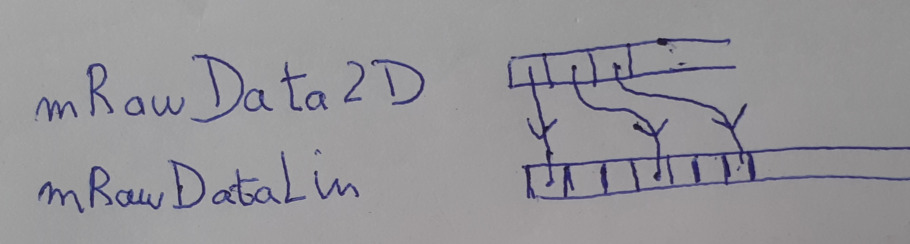
\includegraphics[width=6cm]{Programmer/ImagesProg/PtrIm2D.jpg}
\caption{Structure for {\tt mRawDataXD} vs {\tt mRawDataLin}}
\label{fig:Ptr2D}
\end{figure}

Here is an extract of the initalization of class {\tt cDataIm2D} to better understand
the way it works.


\lstset {language=C++}
\begin{lstlisting}
   for (int aY=Y0() ; aY<Y1() ; aY++)
        mRawData2D[aY] = tBI::mRawDataLin + (aY-Y0()) * SzX() - X0();
\end{lstlisting}


      %  -  -  -  -  -  -  -  -  - - - -  -  -  -  -  -  -  -  - -  -  -  -  -  -  -  -  -  - - - -  -  -  -  -  -  -  -  - -- 

\subsubsection{Methods of class {\tt cDataTypedIm}}

Method  on images that dont rely on the spatial structure between pixels can  advantageously
be implemented using the class {\tt cDataTypedIm} and its field {\tt mRawDataLin} :
it avoid code duplication  and it as fast, if not faster, than implementation using
the {\tt mRawDataXD}. 

For example among many :

\begin{itemize}
    \item {\tt LInfNorm()}  that returns the norm infinite (max of absolute values);

    \item  methods of file  {\tt MMVII\_Tpl\_Images.h} that do not create new images.
\end{itemize}

      %  -  -  -  -  -  -  -  -  - - - -  -  -  -  -  -  -  -  - -  -  -  -  -  -  -  -  -  - - - -  -  -  -  -  -  -  -  - -- 

\subsubsection{Acces to single element}

The methods for read/write single pixel (see ~\ref{GenPixVal}) are
overrided in class {\tt cDataTypedIm}, but they are  not very efficient
as they must convert the point to linear index.

%---------------------------------------------
%---------------------------------------------
%---------------------------------------------

\section{"Final" classes {\tt cDataImXD}}

%----------------------------------------------------------------------------------------
\subsection{Elementary access}

When manipulating images for efficient processing and access to values of pixels, the programmer
will generally use the classes  {\tt cDataImXD}, because these are the classes
that "know" the physicall representation of data. 

The general philosophy for accessing to values is  to have several method to access pixels so that :

\begin{itemize}
    \item  \emph{in mode debug} give a safe access, i.e. all the location are tested (are the point inside
           the definition domain) in read and write, potential overflow are tested in write;

    \item  \emph{in mode release} be as efficient as would be a direct access to raw data;

\end{itemize}

Also the meaning of "extract the value of a pixel"  is different for each dimension $1,2,3$,
and the method must be written for each; however, as much as possible, a unified interface 
give access to value for each dimension.  As these methods are added when needed, they are not
complete for now (i.e many method existing for dimension $2$ are still to write for dimension $3$).
The main methods are :

\begin{itemize}
    \item  \emph{Test:} {\tt Inside} indicate if integer pixel is inside, 

    \item  \emph{access} {\tt GetV,SetV}  for read/write   ,  generate error in mode
           debug if out;

    \item  \emph{safe access} acces with test and no error, {\tt DefGetV} get value with default if out ,
           {\tt SetVTrunc}  modify with truncated value (no error if overflow),
           {\tt SetVTruncIfInside}  modify with truncated values if pixel is inside (no error)

    \item \emph{associative modifier}  {\tt AddVal SetMin SetMax}  update by sum, min or max,


    \item \emph{interpolating}  
      \begin{itemize}
           \item {\tt GetVBL} get value for real pixel using linear interpolation,
           \item {\tt GetGradAndVBL} get value and grad using linear model ;
           \item {\tt InsideBL} inside for linear interpol,
           \item {\tt AddVBL} add value for a real pixel with linear weighting,
           \item {\tt GetValueInterpol, GetValueAndGradInterpol} extract value with a specified interpolator
      \end{itemize}

\end{itemize}

Note that for interpolation there is a generic mode using a specified interpolator and also mode
specialized for linear that are inlined, this version are supposed to be faster when basic linear 
interpolation is sufficient.

%----------------------------------------------------------------------------------------
\subsection{Raw pointer and data organization}

Note also that the class exports also access to raw pointer and {\tt mRawDataXD} , {\tt mRawDataLin}
or a specific line with {\tt GetLine},
these access can be usefull for :

\begin{itemize}
    \item for writing very low level optimization if can be more efficient to work with these
          pointer (even {\tt mRawDataLin} can be used for $2d$ filtering);

    \item for communicating at low-level with external library (this is the used for example
          when using \emph{eigen} and \emph{eigen} in \PPP);

\end{itemize}

Regarding the data organisation for image with dimension $\geq 2$,  the convention
is to access    {\tt mRawData2D[y][x]}  or {\tt mRawData3D[z][y][x]} . This convention
comes from the fact that in image file formats the consecutive pixel are on the same
line (vs the same column). For {\tt mRawDataLin}, the organization is the generalization
of convention of figure~\ref{fig:Ptr2D}, for example :

\begin{equation}
	mRawData3D[z][y][x] = mRawDataLin[x + y * Sz_x + z * Sz_x * Sz_y] \label{EqIm3D}
\end{equation}


%----------------------------------------------------------------------------------------

\subsection{Memory managementi and {\tt cDataImXD} vs {\tt cImXD} }

For safety consideration, it is not possible to creat directly or to copy
the objects of type {\tt cDataImXD} . The way it work is :

\begin{itemize}
	\item the object that can be created are {\tt cImXD}  (i.e {\tt cIm1D, cIm2D, cIm3D })
	\item the {\tt cImXD} are shared pointer to {\tt cDataImXD}, the reference to the {\tt cDataImXD} can
		be extracted via the method  {\tt  DIm()}.
\end{itemize}

%---------------------------------------------
%---------------------------------------------
%---------------------------------------------

\section{Unlimited dimension image}
\label{UlimDimIm}

\PPP propose also a class for images of any dimension. The manipulation is
certainly slower than the specialized version  {\tt cDataImXD}, but can be usefull
for image of dimension $4,5 \dots 10$ for creating a prototype or when performance
is not the main issue.

Basically for these images :

\begin{itemize}
    \item  the constructor take as argument the dimension of the image (i.e. the dimension
	    is not contained in the type, but is a value of the object)

    \item  the access to "pixels" is done via dense vector of type int ({\tt cDenseVect<int>}) ,
	   internaly the data is stored on a linear vector and the conversion is done via
           the generalization of formula like equation \ref{EqIm3D} ;

    \item  access to linear interpolation can also be done via ({\tt cDenseVect<tREAL8>)}), by the
	    way it can be intrinsiqually slow (form dimension D, i.e. there $2^D$ values to access).
\end{itemize}







